\documentclass[letterpaper, 10pt] {article}
\usepackage[margin=0.75in] {geometry}
\title{3D Visualization of Data}
\author{Ryan Sisco - CS461 Fall 2018}
\usepackage{titling}
\usepackage[parfill]{parskip}
\usepackage{graphicx}
\usepackage{float}
\begin{document}
\begin{titlingpage}
	\maketitle
	\vspace*{\fill}
	\begin{abstract}
	When presenting data, it is sometimes difficult to get a grasp on the what it means or what the effects are. There is a need to develop a tool to extract data from files such as location, time, date, names, and others, in order to produce a 3D display. This will help create a better understanding of the data gathered. 
	\end{abstract}
\end{titlingpage}
\section{Problem Description}
Right now there is a problem in malware research where data is collected, but not easily analyzed. There are many open source programs that allow individual points on a 3D globe, but it is a long process. No tools exist to pull the data from CSV files and plot all of that data at once. Adding data points individually wastes time and opens the opportunity for user error when entering data. This also means that in a massive spreadsheet, the user would need to enter the data based on their filter manually. Ultimately, there needs to be a way to take CSV data and populate a 3D globe.
\section{Proposed Solution}
A tool should be created to pull data from a CSV file into a 3D model. Data should be input from a GUI, however, for raw functionality it can be pulled in from a command line just for developmental purposes. Pulling in data will be fairly easy to do, as we have all done it several times in several different computer languages. We imagine this will be done within the first 2 weeks of the assigned project, however, we can continue to pursue a more efficient way to import the data.	Depending on user preference, a graphical interface will be developed to make it easier to choose files and settings. If preferred, it can also allow a console to input commands directly. This all depends on how its priority to the client. 

Data population will be the most challenging part of the project. There are many open source projects that create 3D models of the earth that are able to be populated.	This will take a lot of time to get running in a stable way, that works with our given data. We would also like to add extra features such as color, different 3D models, better interface, etc. This would be developed later on, after the base project is done. 

After the project works with 1 3D model, we can include and create different visualizations. This is all "filler" and can be added non-stop until the project is done. We will reach out and collaborate on renderings that are requested by everyone. One of the most important parts of this assignment is differentiating the data. This project includes adding multiple data points such as dates and malware type. It would be a great addition to add an option to sort colored data by date or malware.
	\begin{figure}[H]
	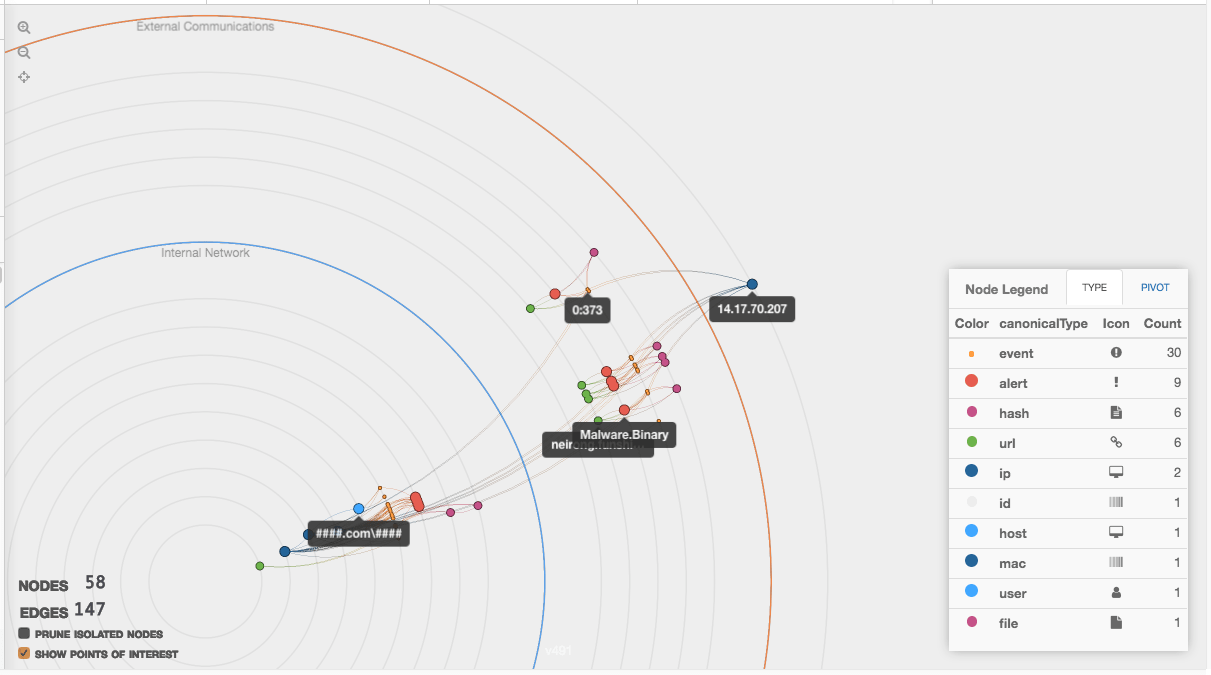
\includegraphics[width=\linewidth]{img/Graph1.png}
	\caption{Malware Graph taken from a resource provided}
	\label{fig:ibm}
	\end{figure}
This is a small example of what is the end goal, as we are planning on a 3D model, but with the same pinpoints and lines shown. This should be flexible and will offer many different visualizations as time allows.
\section{Performance Metrics}
The main deliverable for this project is an application to produce a visual representation of the provided data. This can be achieved by good communication and good organization. If the project stays on track and still falls within the sprint goals, the end result should meet its requirements and prove successful. 

In order to effectively implement our goals, biweekly meetings have been set, one with the client and one with the team. This means we will stay on task and not lose sight of our goals.

Making a user friendly piece of equipment to process the data is essential, and we plan on developing this in the most effective way possible. If it is preferred, we can have it run through command lines, or we can have it use a GUI.   
\end{document}